\documentclass[review]{elsarticle}

\journal{ }

% packages
\usepackage{microtype}
\usepackage{algorithm}
\usepackage[noend]{algpseudocode}
\usepackage[a4paper, total={6.2in, 9in}]{geometry}
\renewcommand{\baselinestretch}{1.2} 
\usepackage{color}
\usepackage[x11names]{xcolor}
\usepackage[utf8]{inputenc}
\usepackage{amsmath}
\usepackage{amssymb,latexsym}
\usepackage{graphicx}
\usepackage{booktabs}
\usepackage{amsfonts}
\usepackage{tikz}
\usepackage{array}
\usepackage{mathtools}
\usepackage{relsize}
\usepackage[T1]{fontenc}
\usepackage{cases}
\usepackage{amsthm}
\usepackage{subcaption}
\usepackage{multirow}
\usepackage{stix2}
\usepackage[labelfont=bf,font=footnotesize]{caption}
\usepackage{tabularx,ragged2e,booktabs}
\usepackage{lineno}
\modulolinenumbers[5]
\usepackage[toc]{appendix}
\usepackage{hyperref}

%new commands
\renewcommand{\figurename}{{Figure}}
\newcolumntype{Y}{>{\centering\arraybackslash}X}
\newtheorem{theorem}{Theorem}
\newtheorem{remark}{Remark}[section]
\numberwithin{equation}{section}
\newcommand{\footremember}[2]{%
    \footnote{#2}
    \newcounter{#1}
    \setcounter{#1}{\value{footnote}}%
}
\newcommand{\footrecall}[1]{%
    \footnotemark[\value{#1}]%
}

\DeclareMathAlphabet{\mathpzc}{OT1}{pzc}{m}{it}
\newcommand{\lnorm}{\left|\left|}
\newcommand{\rnorm}{\right|\right|}
\newcommand{\Ld}{L^2(\mathcal{D})}
\newcommand{\Lomtd}{L^2(\Omega;\mathcal{T};\mathcal{D})}
%\newcommand{\Lomd}{L^2(\Omega;L^2(\mathcal{D}))}
\newcommand{\Lomd}{L^2(\Omega,\mathcal{D})}

% bibliography
\newcommand{\myreferences}{../references,../Mendeley_refs}
\bibliographystyle{abbrv} %elsarticle-num}


\numberwithin{equation}{section}
\graphicspath{{./images/}}

\DeclareMathAlphabet{\mathpzc}{OT1}{pzc}{m}{it}

\pagestyle{myheadings}

%%%%%%%%%%%%%%%%%%%%%%%
\begin{document}

\begin{frontmatter}
\title{A global sensitivity analysis of model uncertainty in aeroelastic wind turbine models}

\address[cwi]{Centrum Wiskunde \& Informatica (CWI), Amsterdam, The Netherlands}
%\address[aero]{Faculty of Aerospace Engineering, Delft University of Technology, Delft, The Netherlands.}
%\author[cwi,aero]{Prashant~Kumar}
\author[]{Prashant~Kumar}\ead{pkumar@cwi.nl}

\author{Benjamin~Sanderse}

\begin{abstract}
Wind turbines are a complex multi-physics systems whose performance and life span is highly dependent on manufacturing, meteorological and operational factors. It is therefore important to quantify the impact of these parameters on the turbine response. We perform comprehensive sensitivity analysis of aeroelastic models typically employed to compute turbine response. This paper also seeks to quantify sensitivities due to manufacturing tolerance in the turbine blades. We propose a non-uniform rational basis splines approach to parametrize the geometry of the blade and further utilize this for quantifying geometric sensitivities at different radial locations. [Some important results]
\end{abstract}
\begin{keyword}
BEM, global sensitivity analysis, model uncertainty, Sobol indices
\end{keyword}
\end{frontmatter}

\linenumbers

\section{Introduction}
Aeroelastic models such as the Blade Element Momentum (BEM) models \cite{HandBook} play a critical role in the design, development and optimization of modern wind turbines. A large number of BEM models have been developed to predict turbine responses such as the structural loads and power output \cite{Vorpahl2013}. 

As a consequence of the strong model assumptions at the basis of BEM theory, the results from BEM codes can be subject to significant inaccuracies or uncertainties. For example, the effect of sheared inflow \cite{Madsen2012} is not naturally accounted for in the theory, and needs to be incorporated via correction terms. Other major model uncertainties in BEM models are for example the time constant in dynamic stall models, the wake correction factor, the tip loss model parameter, and the lift- and drag-polars used to compute local aerodynamic forces. Especially for increasing turbine sizes, these model parameters  are foreseen to be not sufficiently accurate \cite{Sayed2019}. In other words, the uncertainty associated to the output of currently employed BEM models is rather large. 
% iIn order to arrive at robust BEM models that include an uncertainty estimate associated 

Recently, several papers have addressed the uncertainty in BEM model output by performing forward uncertainty propagation or sensitivity studies, e.g.\ \cite{Echeverria2017,Matthaus2017,Murcia2018,Robertson2018,Bos2019a}. In these studies, the focus in mainly on uncertainties in the external conditions (wind parameters) and/or uncertainty in the turbine specification (geometric parameters). Apart from understanding how uncertainty in the output is related to the different uncertain inputs, such sensitivity studies are very useful to reduce the number of parameters as needed for example in design optimization \cite{Echeverria2017}. However, the uncertainty in BEM model output as caused by uncertainty in the model formulation itself, e.g.\ through the values chosen for model parameters, has been given little attention (exceptions being the effect of aerodynamic properties studied in \cite{Bortolotti2019,Matthaus2017}).

The goal of this work is to perform a systematic assessment of the uncertainty in model parameters in BEM models. We approach this by performing a global sensitivity analysis based on the Sobol expansion approach, which decomposes the total variance of the quantity of interest (model output) into contributions from individual parameters and their combinations, similar to \cite{Echeverria2017,Murcia2018,Rinker2016}. We will employ the uncertainty quantification toolbox \texttt{UQLab} \cite{uqlab}, which computes the Sobol indices based on a sparse polynomial chaos expansion. 

Clearly, the main novelty of the work lies in the study of the effect of model uncertainties rather than external conditions or geometric uncertainties. The current sensitivity analysis is part of the so-called WindTrue project, in which the long-term goal is the development of calibrated BEM models, that possess a quantified level of uncertainty. Anticipating on this goal, we are using the NM80 wind turbine model from the Tjaereborg wind farm, for which extensive measurement data is available through the DanAero project \cite{Troldborg2013} and IEA Task 29. The measurement data will enable the calibration step, and our sensitivity analysis will make clear which of the model parameters should be used in the calibration step.

This paper is structured as follows. First, in section \ref{sec:model_description} we give a short description of the BEM model and associated uncertainties. In section \ref{sec:parameterization} the parameterization of the uncertainties is described, and in section \ref{sec:GSA} the global sensitivity analysis methodology. Section \ref{sec:results} discusses the results of the sensitivity analysis for the NM80 turbine test case, and conclusions follow in section \ref{sec:conclusions}.

%A number of parameters describing meteorological and operational conditions as well as manufacturing specifications are needed as inputs for BEM simulations. In this work, we seek to quantify the sensitivities of these input parameters for different turbine responses. In the past a number of sensitivity studies have been performed to understand the influence of input parameters on different turbine response, for e.g. \cite{moriarty2002effect, eggers2003wind, McKay2014, dykes2014sensitivity, Robertson2018}. Many studies have confirmed that the wind parameters especially the wind speed and wind speed standard deviation have the most influence on aerodynamic performance of turbines. For example, in the case of an upstream turbine, the wind speed is most sensitive to power production. Furthermore, wind speed in combination with wind speed standard deviation has a large influence on the power production of turbines operating in the wake of an upstream turbine. Among operational factors, the rotor RPM is the most sensitive to power production. [More on parameter sensitivities on structural loads]
%
%[Sensitivity on the polars as novel element]
%
%[Mention this study is a part of IEA Task29 project]
%
%In this work, we also study the effect of manufacturing tolerances on the turbine response. Usually, there are some discrepancy between the  manufactured and nominally prescribed design of the turbine blade leading to a suboptimal performance. For BEM models, the turbine shape is described as a series of airfoils along the span of the blade where each airfoil shape is computed using the three quantities: chord length, thickness and twist. We perturb these three quantities to obtain a perturbed turbine blade and analyze with sections that have more influence on output quantities. 
%
%To compute parameter sensitivities we use the Sobol expansion approach, which decomposes the total variance of the quantity of interest into contributions from individual parameters and their combinations. To perform Sobol analysis, we use Matlab-based general purpose uncertainty quantification toolbox \texttt{UQLab} \cite{uqlab}. \texttt{UQLab}'s modular structure allows for easy integration with available BEM codes. For investigation the aeroelastic model of the  2MW NM80 turbine (with an 80m rotor) from the DANAERO project \cite{DANAERO} is utilized.

\section{Aeroelastic models}\label{sec:model_description}
\subsection{BEM model uncertainties}
State-of-the-art wind-turbine models simulate the aeroelastic behavior of wind turbines by combining the concept of momentum conservation of the flow (BEM) with the equations of motion for the structure, possibly extended with hydrodynamics of the sea and control algorithms \cite{Vorpahl2013}. In this work, we only concentrate on the first aspect, namely the prediction of flow and blade forces as given by the BEM method. The particular BEM code that we use is  ECN's \texttt{Aero-Module} \cite{Boorsma2012}.

For this case of a rigid turbine, with a uniform inflow field, the main model uncertainties that arise in the BEM formulation that we will discuss in this work are the following \cite{Hansen1993}:
\begin{itemize}
\item The use of (2D) \textit{airfoil polars}; uncertainty arises not only because the actual flow along the blade is 3D, but also because the 2D polars itself can be inaccurate, either when obtained from measurement or from 2D codes like \texttt{XFOIL};
%\item Sheared inflow
\item The assumption of locally 2D flow along the blade is also invalid at the tip; this is typically corrected via \textit{a tip loss model};
\item Three-dimensional flow effects also cause stall delay at the root; this is typically modelled via \textit{a dynamic stall model }and time constant;
\item Yawed inflow is not naturally included in BEM and typically incorporated via \textit{a wake correction}.

%\item Dynamic wake - Oye time lag constant
%\item Tower shadow constants – Potential flow / Downwind Empirical model

\end{itemize}

%\subsection{Input parameters of aeroelastic models}
%The main 

\section{Parametrization of uncertain inputs in the BEM model}\label{sec:parameterization}

\subsection{Geometric uncertainty}
We use Non-Uniform Rational Basis Splines (NURBS) \cite{rogers2000} to perturb the geometrical parameters of the turbine blade, such as the reference chord, twist or experimentally obtained drag-, lift-polar curves. The main advantage of using NURBS is that it provides great flexibility to approximate a large variety of curves with a limited number of control points which can be useful in reducing the number of uncertain parameter. %Further, the set of control points and knots can be directly manipulated to control the smoothness and curvature.
Use of NURBS has already been exploited in many aerodynamics applications, for instance, design optimization of wind-turbine blades, see for e.g. \cite{Ribeiro2012,Bottasso2014} and to parametrize chord and twist curves \cite{Echeverria2017}. In the following, we briefly outline the procedure used to parametrize curves using NURBS.
\subsubsection{NURBS based perturbation}
The value of NURBS curve at each location $x$ is computed using a weighted sum of $n$ basis functions (or B-splines):
\begin{equation}\label{NURB_curve}
S(x)  = \sum_{i=1}^{n} c_i B_{i,p}(x),
\end{equation}
where $S(x)$ is the value of the NURBS curve at location $x$; $c_i$ is the weight of the $i$-th control point and $B_{i,p}(x)$ is the value of B-spline corresponding to the $i$-th control point at $x$ with the subscript $p$ denoting its polynomial degree. A sequence of non-decreasing parameters $X = \{x_1,x_2,...,x_m\}$ called the \textit{knot vector} determines the domain in which any control point is active with the number of elements in the knot vector is given by $m = n+p+1$. B-splines are non-zero only within a knot interval $[x_i,x_{i+1})$ for $i = 1, 2, ..., m-1$ and are zero elsewhere. Therefore, only a few nearby control points are active when computing the NURBS curve \eqref{NURB_curve}. For a curve of polynomial degree $p$, there are $p+1$ active control points at any location $x$, for e.g., for a linear curve ($p=1$) only two adjacent control points are active at any location. Also, note that the number of B-splines are equal to the number of elements in $X$. Another useful property of the B-splines is that they are recursive in polynomial degree thus we can derive quadratic B-splines using linear B-splines, cubic from quadratic B-splines and so on. Starting with B-spline of degree 0 defined as 
\begin{equation}\label{linearBspline}
B_{i,0}(x) :=
\begin{cases}
1\quad x_i\leq x < x_{i+1},\quad i = 1,2,...,m,\\
0\quad\text{elsewhere,}
\end{cases} 
\end{equation}
we can derive higher order B-splines in the knot interval $[x_{i+p},x_{i+p+1})$ using the recurrence relation \cite{deBoor}:
\begin{equation}\label{NURBS_recurrence}
B_{i,p}(x) := \frac{x - x_i}{x_{i+p} - x_i}B_{i,p-1}(x) + \frac{x_{i+p+1}  -  x}{x_{i+p+1}  -  x_{i+1}}B_{i+1,p-1}(x),\quad p\geq1.
\end{equation} 
These B-splines can be constructed efficiently using the de Boor's algorithm \cite{deBoor}. Note that to perform above computation, we need to pad the knot vector $X$ by repeating the first and last elements $p$ times each. In Fig. \ref{B-splines}, we show linear, quadratic and cubic splines for $x\in[0,1]$ [Also show the padding]. 

Next, we describe steps to generate perturbed samples of chord from a given reference chord, $S_{ref}(x)$, using NURBS based parametrization. The first step is to approximate the given reference chord using a NURBS curve with a fixed degree $p$ and a limited number of knots $X =\{x_j\}_{j=0}^n$. The knots can be uniformly spaced or chosen heuristically, more advanced approaches for knot selection can be found in, for e.g. \cite{razdan1999knot,LI2005791}. Next we sample $S_{ref}(x)$ at $X$ and also compute $B_{i,p}(x_j), \text{ for }i, j = 1,2, ..., n$.  Now we can formulate a linear system to solve for a set of control points $\mathbf{c}=\{c_i\}_{i=0}^n$ as:
\begin{equation}\label{nurbs_inversion}
\mathbf{B}\mathbf{c} = \mathbf{S}_{ref},
\end{equation}
where $\mathbf{S}_{ref}\in\mathbb{R}^{n}$ is a vector containing sampled values of $S_{ref}(x)$ and $\mathbf{B}\in \mathbb{R}^{n\times n}$ is a matrix with $j$-th row consisting of values of $n$ B-splines sampled at the location $x_j$. Once the control points are obtained, we can derive the approximate reference curve $S_n(x)$ using \eqref{NURB_curve}. In this work, we use uniform random variable to perturb the baseline control points $\mathbf{c}$.
 
There are two ways to obtain perturbed curves either by independently perturbing each of the control points (local perturbation) or using the same random number to perturb all the control points (global perturbation). We use local perturbation for chord control points Ch1-Ch5 and twist control points Tw1-Tw6 control points, see Fig. \ref{perturbed_samples} (a) - (b), respectively. Each control points are perturbed using a uniform random number with bounds given by $\pm5\%$ of the magnitude of control point. For lift and drag curve, all control points are perturbed using same uniform random number resulting in samples of the lift and drag curves as shown in Fig. \ref{perturbed_samples} (c) - (d), respectively. For simplicity, we only consider uniform distributions for perturbing the control points, however, we can also use other probability distributions for this. Also note that when using a uniform distribution with bounds given by relative magnitude of control points, we tend to obtain small perturbations for control points with values close to zero.
\begin{figure}[h!]
\centering
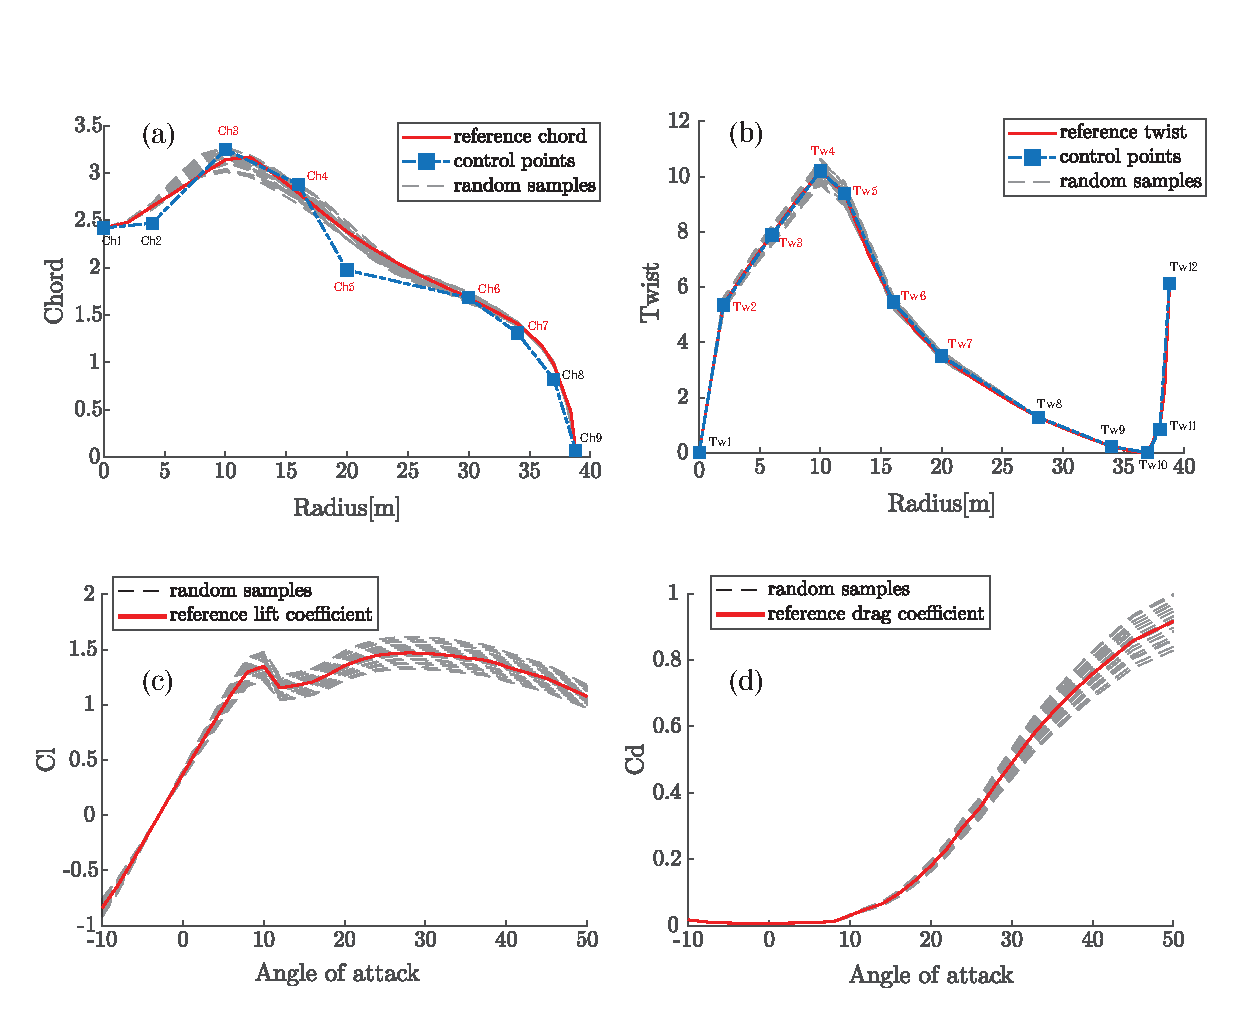
\includegraphics[trim={0 1.6cm 0 1.5cm},clip, scale=0.67]{figure1.pdf}
\caption{Random realization of chord, twist, lift- (Cl2) and drag-polars (Cd2).}
\label{perturbed_samples}
\end{figure}

\section{Global sensitivity analysis}\label{sec:GSA}
The objective of sensitivity analysis is to quantify the relative significance of individual inputs (or in combination) and how variations in input values affects the output of interest. In engineering, sensitivity analysis can be employed for a number of reasons: to determine the stability and robustness of a computational model with respect to input parameters, for simplification of stochastic models by fixing the insensitive parameters, and to guide data acquisition campaigns and experimental design to refine the data on sensitive parameters. Sensitivity analysis techniques can be classified as local and global methods, see \cite{RSmith}. In local sensitivity analysis, individual parameters are perturbed around their nominal values allowing for the description of output variability only in a small neighbourhood of nominal input values. Although, local approaches are widely employed due to their ease of implementation and low computational cost, they are unable to quantify global behavior of nonlinearly parametrized models such as aeroelastic models. Global sensitivity approaches, on the other hand, consider the entire range of input values to compute output sensitivities. Therefore, global sensitivity analysis is more suitable for aeroelastic models considered in this work.  

\subsection{Sobol analysis}
We employ variance-based Sobol decomposition to perform global sensitivity analysis. This approach allows for quantification of  the relative importance of the input parameters on a scale of $[0,1]$ known as \emph{Sobol indices}. In a Sobol analysis, we express the total variance of the output in term of contributions from individual parameters and their combinations. For the ease of exposition, let us consider a nonlinear model:
\begin{equation}\label{nonlinear_model}
Y = f({\mathbf{z}}),
\end{equation}
where ${\mathbf{z}} = [z_1, z_2, ..., z_M]\in \mathcal{D}_{\mathbf{z}}\in \mathbb{R}^M$ is a vector of random  inputs. For simplicity, we assume input parameters are uniformly distributed i.e. $z_i \sim \mathcal{U}(0,1)$ and the support of input set is $\mathcal{D}_{\mathbf{z}}  =  [0,1]^M$ where $M$ is the total number input parameters. The Sobol decomposition is based on the hierarchical representation \cite{RSmith}:
\begin{equation}\label{sobol_decomp}
f(z_1, z_2, ..., z_M) = f_0+\sum_{i=1}^M f_i(z_i) + \sum_{1\leq<i<j\leq M} f_{ij}(z_i,z_j) + ... + f_{1, 2, ..., M}(z_1, z_2, ..., z_M),
\end{equation}
where the zeroth-order function $f_0$ is the mean response of $f$, the first-order univariate functions $f_i(z_i)$ quantify independent contributions due to each random input, second-order functions $f_{i,j}(z_i,z_j)$ represent the effect of interaction between $z_i$ and $z_j$ on the response $f$. Note that the \eqref{sobol_decomp} is only valid for independent input parameters. Higher-order terms are interpreted in a similar manner. Formally, the zeroth-, first- and second-order terms are defined as:
\begin{align}\label{sobol_terms}
f_0 &= \int_{\mathcal{D}_{\mathbf{z}}}f(\mathbf{z})d\mathbf{z},\\
f_i(z_i) &= \int_{{\mathcal{D}_{\mathbf{z}}}^{M-1}}f(\mathbf{z})d\mathbf{z}_{\sim \{i\}} - f_0,\\
f_{ij}(z_i,z_j) &= \int_{{\mathcal{D}_{\mathbf{z}}}^{M-2}}f(\mathbf{z})d\mathbf{z}_{\sim \{i,j\}} - f_i(z_i)  - f_j(z_j) - f_0,
\end{align}
where ${\mathcal{D}_{\mathbf{z}}}^{M-1} = [0,1]^{M-1}$ and the notation $\mathbf{z}_{\sim \{i,j\}}$ denotes the vector having all the components of $\mathbf{z}$ except in the set $\{i,j\}$. We only consider second order expansion of \eqref{sobol_decomp}, as for a number of applications, the second order expansion is usually sufficient and higher-order terms have negligible effect on the output response. In case of wind turbine, suppose $y$ represent the power output that depends on say 3 random inputs:  windspeed $(z_1)$, wind standard deviation $(z_2)$ and RPM $(z_3)$, then $f_0$ represents the mean power output considering all the three random inputs, $f_1(z_1)$ represent the independent contribution of windspeed on the power and $f_{1,2}(z_1,z_2)$ quantify the interactions of wind speed and wind standard deviation on power. Further, the total variance of $f(\mathbf{z})$ is defined as:
\begin{equation}\label{tot_var}
D = \text{Var}[f(\mathbf{z})] = \int_{\mathcal{D}_{\mathbf{z}}} f^2(\mathbf{z})d\mathbf{z} - f_0^2
\end{equation}
As the expansion in \eqref{sobol_decomp} is not unique, some orthogonality conditions must be imposed, see \cite{Rabitz1999,SOBOL2001271} which allows to express the total variance as
\begin{equation}
D = \sum_{i=1}^M D_i + \sum_{1\leq i<j\leq M} D_{ij},
\end{equation}
where the first- and second-order partial variances are defined as
\begin{align}
D_i &= \int_{0}^{1} f^2_i(z_i)dz_i, \label{partial_variance1}\\
D_{ij} &= \int_{0}^{1} \int_{0}^{1} f^2_{ij}(z_i,z_j)dz_idz_j \label{partial_variance2}. 
\end{align}
The first- and second-order Sobol indices are computed as
\begin{equation}\label{sobol_ind}
S_i = \frac{D_i}{D}, \quad  S_{ij} = \frac{D_{ij}}{D}, \quad i,j=1,2, ..., M,
\end{equation}
and the sum of all indices satisfy
\begin{equation}
\sum_{i=1}^M S_i + \sum_{1\leq i<j\leq M} S_{ij} = 1.
\end{equation}
Finally, the total effect of the parameter $z_i$ on the output response $Y$ is quantified using the total sensitivity indices measure
\begin{equation}
S_{T_i} = S_i + \sum_{j=1}^M S_{ij}.
\end{equation}
The total sensitivity indices can be interpreted as an importance measure for the parameter $z_i$, therefore a large $S_{T_i}$ implies that $z_i$ has a strong influence on $Y$. The computation of $S_{T_i}$ requires the approximation of partial variances defined in \eqref{partial_variance1} - \eqref{partial_variance2}. Using the Monte Carlo method for computing these variance can be prohibitive for computationally expensive models $Y$.  Polynomial Chaos Expansions (PCE) based approaches provides a more efficient alternative for sensitivity analysis. As shown in \cite{SUDRET2008964}, one can compute the Sobol indices analytically by post-processing the PCE coefficients.
\subsection{PCE based Sobol indices computation}
The PCE $f^{K}(\mathbf{z})$ of the computational model $Y$ is defined as a weighted sum of multivariate polynomials in $\mathbf{z}$ \cite{RSmith}
\begin{equation}
Y = f^{K}(\mathbf{z}) = \sum_{|\mathbf{k}| = 0}^K y_{\mathbf{k}}\Psi_{\mathbf{k}}(\mathbf{z}),
\end{equation}
where $\mathbf{k}\in  \mathbb{N}_0^M$ is a $M$-dimensional multi-index with the magnitude $|\mathbf{k}| = k_1+k_2 + ... + k_M$, whereas $\Psi_{\mathbf{k}}(\mathbf{z})$ is the multivariate orthogonal polynomials that is computed using a tensor product of univariate polynomials $\psi_{k_i}^{(i)}(z_i)$
\begin{equation}
\Psi_{\mathbf{k}}(\mathbf{z}) := \prod_{i=1}^M\psi_{k_i}^{(i)}(z_i).
\end{equation}
The choice of the univariate orthogonal polynomial $\psi_{k_i}$ depends on the type of random variable, $z_i$. For example, if for uniformly distributed random variable, the Legendre family of polynomials is used, see  \cite{Xiu2002} for details. Projection methods are typically employed for the calculation 

Quadrature based integration methods suffer from curse of dimensionality where the number of integration points rises exponentially with an increase in the number of dimensions. For applications with a fixed computational budget methods that minimizes the approximation error with a given number of samples are usually more practical. Next, we briefly describe two such methods to compute PCE coefficients based on a given number of model evaluations.

\subsubsection{Ordinary Least Square}
The 
\subsubsection{Least Angle Regression (PCE\_LAR)}
\subsection{Sensitivity analysis with discrete random variable}
%\section{Description of test case}
%\section{Sensitivity analysis workflow}
\section{Results}\label{sec:results}

\subsection{NM80}
 and the turbine is the 2MW NM80 turbine from the DANAERO project \cite{Troldborg2013} with a blade radius of 38.8m. The data for lift ($Cl$) and drag ($Cd$) polars are available at four locations along the blade radius at 11.87m, 17.82m, 28.97m and 35.53m. The reference value of polars are obtained from wind-tunnel experiment with 3D corrections. Random samples of chord, twist, lift- and drag-polars are obtained by perturbing the control points with a uniformly distributed random variable. For chord and twist, we independently perturb control points at different locations as shown in Fig. \ref{fig:samples} (a) - (b). For $Cl$ and $Cd$, all control points are perturbed using a same random number.
 
\subsubsection{Verification of GSA method}
Convergence study of UQLab with increasing number of samples for Quad, OLS, LARS.

\subsection{AVATAR}

\section{Conclusions}\label{sec:conclusions}

\section*{Acknowledgements}

\newpage
\bibliography{\myreferences}

\newpage

\appendix
\section{Literature overview of global sensitivity analysis in wind-turbine models}
List of BEM codes in \cite{Sayed2019,Vorpahl2013}.

Uncertainties and corrections in BEM models \cite{Madsen2012}: complex inflow, e.g. sheared inflow.

\cite{Eggers2003} study the effect of shear and turbulence on rotor loading, but not with a systematic (global) sensitivity analysis.

\cite{McKay2014} perform a measurement data-only global sensitivity analysis using a neural network and a Fourier amplitude sensitivity test (a similar technique was used in \cite{Kusiak2010} for vibration analysis). The neural network is constructed based on measurement data. The output quantity of interest is the power production; several input parameters are used, including yaw angle, rotor speed, blade pitch angle, wind speed, ambient temperature, main bearing temperature, wind speed standard deviation and yaw angle standard deviation.

\cite{Dykes2014} performed global sensitivity analysis of turbine costs with respect to key wind turbine configuration parameters including rotor diameter, rated power, hub height, and maximum tip speed. DAKOTA is used to calculate Sobol indices with Monte Carlo sampling.

\cite{Rinker2016a} calculated the global sensitivity of wind turbine loads to wind inputs using polynomial response surfaces. She used Sobol indices, with quantity of interest the maximum blade root bending moment and as inputs four turbulence parameters: a reference mean wind speed, a reference turbulence intensity, the Kaimal length scale, and a parameter reflecting the nonstationarity. The turbine model studied is the WindPACT 5 MW reference model and the BEM model is FAST.

\cite{Echeverria2017} employs a global sensitivity analysis to identify the design variables that affect wind turbine performance in order to reduce the number of variables in wind turbine design optimization. As input parameters, airfoil parameterization and chord and twist distributions are used; the outputs studied are annual energy production, maximum blade tip deflection, overall sound power level and blade mass. For example, Sobol indices are shown for the effect of chord and twist control points on the output quantities.

\cite{Matthaus2017} performed uncertainty quantification including uncertainty in the aerodynamic properties; for example, the uncertainty in the lift coefficient at an airfoil section due to uncertain roughness (e.g.\ contamination) is achieved by interpolating between clean and fully rough state with a uniformly distributed random variable. Polynomial chaos and Kriging were used. See also \cite{Bortolotti2019}, in which the AVATAR turbine was analysed, using the Cp-Lambda aeroelastic model and DAKOTA as UQ toolbox. 

\cite{Murcia2018} similarly considered a global sensitivity analysis with Sobol indices computed by using sparse polynomial chaos expansion. The quantities of interest considered are the energy production and lifetime equivalent fatigue loads for the DTU 10 MW reference turbine. The uncertain input is given by the turbulent inflow field, with 4 parameters: mean hub height wind speed, std. dev. of hub height wind speed, shear exponent, yaw misalignment. The dependency between these parameters (as described by the Normal Turbulence Model) is taken into account by using a Rosenblatt transformation that transforms the dependent variables to a set of independent ones. The Chaospy package is used for the analysis. Seven different model outputs are considered: power, thrust, and several damage equivalent fatigue loads (EFL), computed using a rainflow counting algorithm. The sensitivity analysis shows that the turbulent inflow realization has a bigger impact on the total distribution of equivalent fatigue loads than the shear coefficient or yaw misalignment.

\cite{Sayed2019} argue that BEM models are accurate mainly for small turbines but that for large turbines, when the tip deformations exceed 10\% of the blade radius, it is questionable if they can still be applied. They compare the results of engineering models to CFD-based aeroelastic simulations. It is shown that the 2D polars commonly used in BEM require 3D corrections, and that including more polars improves the results. `Turbine power and thrust predicted from the flexible rotor were reduced compared to the rigid rotor employing a BEM-based model. A reason behind the increase in power from the CFD-based model is the spanwise force component. It is not included in the BEM-based simulations as it is one of the main assumptions of its theory. This assumption could be used for small wind turbine simulations where the edgewise deformations were insignificant. But for such large wind turbines, the spanwise force distribution over the blade radius must be taken into account in the calculation of the power output due to the large edgewise deformations. To increase the accuracy of the engineering model, it is recommended to increase the number of polars calculated by 2D CFD simulations at different sections along the blade. This is because of the significant difference in the Reynolds number for the large blade.'

\cite{Velarde2019} perform a global sensitivity analysis of fatigue loads with respect to structural, geotechnical and metocean parameters for a 5MW offshore wind turbine installed on a gravity based foundation. Linear regression of Monte Carlo simulations and Morris screening are performed for three design load cases. 

\cite{Robertson2018} assesses the sensitivity of different wind parameters on the loads of a wind turbine. They argue that the most common parameters considered normally in literature are the turbulence intensity variability, and the shear exponent, or wind profile, both having important influence on the turbine response. In the paper an assessment of which wind characteristics influence wind turbine structural loads is given. The correlated dependency between the individual parameters is not considered; rather, they focus on assessing the sensitivity of each parameter individually. An elementary-effects screening method (Morris screening) is used as global sensitivity method. The NREL 5MW turbine and FAST are used.

\cite{Fluck2018} develop an \textit{intrusive} stochastic BEM method: `a stochastic solution for the unsteady aerodynamic loads based on a projection of the unsteady Blade Element Momentum (BEM) equations onto a stochastic space spanned by chaos exponentials'.

\cite{Hubler2017} used global sensitivity analysis (as part of a four-step approach) to reduce the parameter dimension for structural behaviour computations using FAST as aeroelastic code. The methods of expert knowledge, one-at-a-time variation, and regression based on Monte Carlo sampling are used as pre-processing steps to reduce the computational expense of global sensitivity analysis.

\end{document}